\begin{figure}[ht]
  \centering
  \caption{\label{fig:api_docs}The API documentation generated by Swagger UI}
  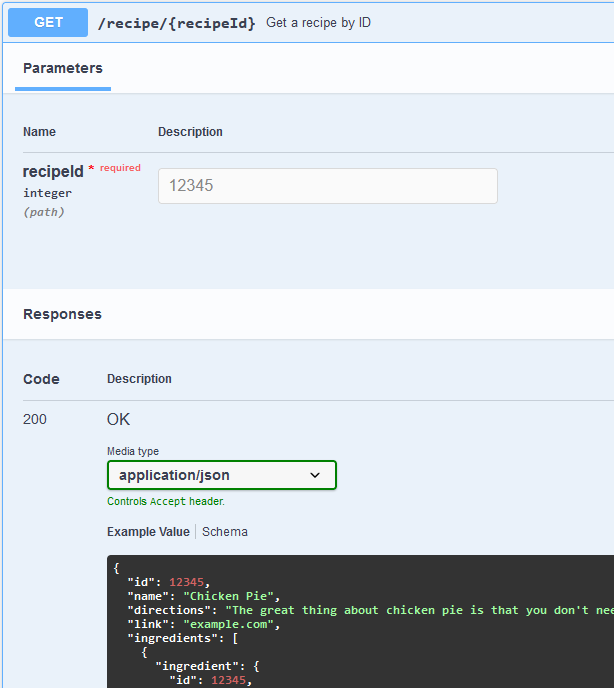
\includegraphics[width=\columnwidth]{figures/api_docs_example.png}
\end{figure}

\begin{figure}[ht]
  \centering
  \caption{\label{fig:importer_schema}The parts of the schema used during import}
  \begin{tikzpicture}
    \begin{class}{Embedding}{0,4}
      \attribute{+ sentence: string}
      \attribute{+ embedding: Float32Array}
    \end{class}

    \begin{class}{Recipe}{0,0}
      \attribute{+ id: int}
      \attribute{+ name: string}
      \attribute{+ directions: string}
      \attribute{+ link: string}
      \attribute{+ mealTypeId: int}
    \end{class}
    \association{Recipe}{name}{1}{Embedding}{sentence}{1..*}

    \begin{class}{MealType}{9,2}
      \attribute{+ id: int}
      \attribute{+ name: string}
    \end{class}
    \association{Recipe}{mealTypeId}{1}{MealType}{id}{0..*}
    \association{MealType}{name}{1}{Embedding}{sentence}{1..*}

    \begin{class}{Ingredient}{9,-5}
      \attribute{+ id: int}
      \attribute{+ name: string}
      \attribute{+ assumeUnlimited: bool}
      \attribute{+ preferredUnit: string}
      \attribute{+ density: float|null}
    \end{class}

    \begin{class}{RecipeIngredient}{0,-5}
      \attribute{+ recipeId: int}
      \attribute{+ ingredientId: int}
      \attribute{+ amount: float|null}
      \attribute{+ originalLine: string}
    \end{class}
    \association{Recipe}{id}{1}{RecipeIngredient}{recipeId}{0..*}
    \association{Ingredient}{id}{1}{RecipeIngredient}{ingredientId}{0..*}

  \end{tikzpicture}
\end{figure}

\clearpage\subsection{Sequence Diagrams}\label{sec:sequence_diagrams}

\begin{figure}[ht]
  \centering
  \caption{\label{fig:add_manual}The sequence diagram for adding ingredients manually.}
  \begin{sequencediagram}
      \newthread{user}{:User}
      \newinst[1]{web}{:Web App}
      \newinst[1]{api}{:API}

      \begin{call}{user}{Open Form}{web}{}
          \begin{call}{web}{Fetch Ingredients}{api}{}
          \end{call}
          \begin{call}{web}{Select Ingredient}{user}{}
          \end{call}
          \begin{call}{web}{Select Amount}{user}{}
          \end{call}
          \begin{call}{web}{Update Amount}{api}{}
          \end{call}
      \end{call}
  \end{sequencediagram}
\end{figure}

\begin{figure}[ht]
  \centering
  \caption{\label{fig:add_barcode}The sequence diagram for adding ingredients by scanning a barcode.}
  \begin{sequencediagram}
      \newthread{user}{:User}
      \newinst[1]{web}{:Web App}
      \newinst[1]{scanner}{:Barcode Library}
      \newinst[1]{api}{:API}

      \begin{call}{user}{Scan Barcode}{web}{}
          \begin{call}{web}{Decode Barcode}{scanner}{}
          \end{call}
          \begin{call}{web}{Fetch Ingredient}{api}{}
          \end{call}
          \begin{call}{web}{Confirm}{user}{}
          \end{call}
          \begin{call}{web}{Update Amount}{api}{}
          \end{call}
      \end{call}
  \end{sequencediagram}
\end{figure}

\begin{figure}[ht]
  \centering
  \caption{\label{fig:add_receipt}The sequence diagram for adding ingredients by scanning a receipt.}
  \begin{sequencediagram}
      \newthread{user}{:User}
      \newinst[1]{web}{:Web App}
      \newinst[1]{ocr}{:OCR API}
      \newinst[1]{api}{:API}

      \begin{call}{user}{Scan Receipt}{web}{}
          \begin{call}{web}{Extract Text}{ocr}{}
          \end{call}
          \begin{call}{web}{Parse Ingredients}{api}{Ingredients and Amounts}
          \end{call}
          \begin{call}{web}{Confirm}{user}{}
          \end{call}
          \begin{call}{web}{Update Amounts}{api}{}
          \end{call}
      \end{call}
  \end{sequencediagram}
\end{figure}

\begin{figure}[ht]
  \centering
  \caption{\label{fig:change_preferences}The sequence diagram for changing user preferences.}
  \begin{sequencediagram}
    \newthread{user}{:User}
    \newinst[1]{web}{:Web App}
    \newinst[1]{api}{:API}

    \begin{call}{user}{Open Preferences}{web}{}
      \begin{call}{web}{Fetch Current}{api}{}
      \end{call}
      \begin{call}{web}{Update Preferences}{user}{New Preferences}
      \end{call}
      \begin{call}{web}{Apply Changes}{api}{}
      \end{call}
    \end{call}
  \end{sequencediagram}
\end{figure}

\begin{figure}[ht]
  \centering
  \caption{\label{fig:find_recipe}The sequence diagram for finding recipes.}
  \begin{sequencediagram}
      \newthread{user}{:User}
      \newinst[1]{web}{:Web App}
      \newinst[1]{api}{:API}

      \begin{call}{user}{Search}{web}{}
        \begin{call}{web}{Select Meal Type}{user}{}
        \end{call}
        \begin{call}{web}{Select Filters}{user}{}
        \end{call}
        \begin{call}{web}{Fetch Recipes}{api}{}
        \end{call}
      \end{call}
      \begin{call}{user}{View Recipe}{web}{}
        \begin{call}{web}{Fetch Details}{api}{}
        \end{call}
        \begin{call}{web}{Fetch Related}{api}{}
        \end{call}
      \end{call}
  \end{sequencediagram}
\end{figure}

\begin{figure}[ht]
  \centering
  \caption{\label{fig:made_recipe}The sequence diagram for marking a recipe as made.}
  \begin{sequencediagram}
      \newthread{user}{:User}
      \newinst[1]{web}{:Web App}
      \newinst[1]{api}{:API}
      \newinst[1]{db}{:Database}

      \begin{call}{user}{Mark Made}{web}{}
        \begin{call}{web}{Update History}{api}{}
          \begin{call}{api}{Append History}{db}{}
          \end{call}
          \begin{call}{api}{Deduct Ingredients}{db}{}
          \end{call}
        \end{call}
      \end{call}
  \end{sequencediagram}
\end{figure}

\clearpage\subsection{Interface Prototypes}

\begin{figure}[ht]
  \centering
  \includesvg[height=0.89\textwidth,width=0.7\textheight,angle=90,pretex=\relscale{0.6}]{figures/InterfacePrototypes}
  \caption{\label{fig:proto_fridge}The fridge page for \chef{}, allowing the user to add/remove ingredients and scan items.}
\end{figure}

\begin{figure}[ht]
  \centering
  \includesvg[height=0.9\textwidth,angle=90,pretex=\relscale{0.8}]{figures/FindRecipePage}
  \caption{\label{fig:proto_find_recipes}The find recipes page, showing recipes that can be made by the user. }
\end{figure}

\begin{figure}[ht]
  \centering
  \includesvg[height=0.9\textwidth,angle=90,pretex=\relscale{0.8}]{figures/AccountPage}
  \caption{\label{fig:proto_account}The account page, allowing the user to change their preferences.}
\end{figure}

\clearpage\subsection{Code Snippets}

\begin{figure}
  \caption{\label{fig:type_check}A code snippet that would fail TypeScript's checks.}
  \begin{minted}{ts}
function take_str(str: string): void {
  console.log(str)
}

// This would compile, as it is passed the expected type
take_str('Hello')

// This would not compile as take_str expects a string,
// but a number was passed
take_str(123)

// This would also not compile as take_str does not return
// anything
const ret = take_str('World')
  \end{minted}
\end{figure}

\begin{figure}[h]
  \centering
  \caption{\label{fig:buffer_float_array}The test case for round trip accuracy between buffers and float arrays}
  \begin{minted}{ts}
it('should convert a Float32Array to a Buffer and back without changes',
  // Generate some random data
  () => {
    const input = Float32Array.from(
      { length: 10 }, () => faker.number.float({ min: 0, max: 1 })
    )

    // Convert it to a buffer and back again
    const buffer = bufferFromFloat32Array(input)
    const output = bufferToFloat32Array(buffer)

    // Check that the output is identical
    assert.deepStrictEqual(output, input)
})
  \end{minted}
\end{figure}

\cleartoleftpage\begin{figure}
  \centering
  \caption{\label{fig:search_query}The query used to search recipes}
  % cSpell: disable
  \begin{minted}{sql}
SELECT
recipe.name, recipe.id,
-- COUNT excludes NULLs.
COUNT(
  CASE
    -- If fridgeId is null, then we can't
    -- create a meaningful missing count
    WHEN :fridgeId IS NULL THEN NULL

    -- Check if we have any of the ingredients
    WHEN fridge_ingredient.amount IS NULL THEN 1

    -- Optionally check if we have enough of the ingredients
    WHEN
      :checkAmount AND
      fridge_ingredient.amount < recipe_ingredient.amount
      THEN 1
  END) as missing_count,
CASE WHEN :search IS NULL
  THEN NULL
  ELSE ml_similarity(embedding.embedding, :search)
END AS similarity
FROM recipe
JOIN embedding ON embedding.sentence = recipe.name
LEFT JOIN recipe_ingredient ON
  recipe_ingredient.recipe_id = recipe.id
LEFT JOIN fridge_ingredient ON
  fridge_ingredient.ingredient_id = recipe_ingredient.ingredient_id
    AND
  fridge_ingredient.fridge_id = :fridgeId
JOIN ingredient ON
  ingredient.id = recipe_ingredient.ingredient_id AND
  NOT ingredient.assumeUnlimited
LEFT JOIN ingredient_tag ON
  ingredient_tag.ingredient_id = ingredient.id
WHERE (
  recipe.meal_type_id = (
    SELECT id FROM meal_type WHERE name = :mealType
  ) OR :mealType IS NULL
) AND (similarity >= :minSimilarity OR :search IS NULL)
GROUP BY recipe.id
  \end{minted}
\end{figure}

\begin{figure}\ContinuedFloat{}
  \begin{minted}{sql}
HAVING
(missing_count <= :maxMissingIngredients OR :fridgeId IS NULL)
-- SUM(CASE WHEN ... THEN 1 ELSE 0 END) = 0
-- checks for CASE WHEN returning false for all rows
-- No banned tags
AND (SUM(CASE WHEN
  ingredient_tag.tag_id IN
    (SELECT tag_id FROM ${bannedTagsTable})
THEN 1 ELSE 0 END) = 0)
-- No banned ingredients
AND (SUM(CASE WHEN
  recipe_ingredient.ingredient_id IN
    (SELECT ingredient_id FROM ${bannedIngredsTable})
THEN 1 ELSE 0 END) = 0)
ORDER BY missing_count ASC, similarity DESC
LIMIT :limit
  \end{minted}
  % cSpell: enable
\end{figure}

\cleartoleftpage\begin{figure}
  \caption{\label{fig:search_params}The parameters of the \texttt{search} endpoint}
  \begin{minted}{yaml}
- in: query
  name: search
  description: Search term
  schema: { type: string, example: "chicken pie" }
  required: false
- in: query
  name: minSimilarity
  description:
    Minimum similarity score,
    meaningless if `search` is not specified
  schema:
    type: number
    example: 0.5
    minimum: 0
    maximum: 1
    default: 0.5
  required: false

- in: query
  name: availableForFridge
  description:
    If specified, only return recipes that can be
    made with the ingredients in the fridge.
  schema: { $ref: "#/components/schemas/id" }
  required: false
- in: query
  name: maxMissingIngredients
  description:
    Maximum number of ingredients that can be missing.
    Meaningless if `availableForFridge` is not specified.
  schema:
    type: integer
    minimum: 0
    example: 1
    default: 0
  required: false
- in: query
  name: checkAmounts
  description:
    Whether to check that there is enough of each ingredient.
    Meaningless if `availableForFridge` is not specified.
  schema: { type: boolean, example: true, default: true }
  required: false
  \end{minted}
\end{figure}

\begin{figure}\ContinuedFloat{}
  \begin{minted}{yaml}
- in: query
  name: limit
  description: Maximum number of results to return.
  schema:
    type: integer
    example: 10
    minimum: 1
    default: 10
  required: false
- in: query
  name: mealType
  description:
    If specified, only return recipes of this type.
    By default, all recipes are returned.
  schema: { type: string, example: "Dinner" }
  required: false

- in: query
  name: suitableForUsers
  description:
    If specified, only return recipes that are suitable for
    all of these users considering their dietary restrictions.
    By default, no restrictions are applied.
  schema:
    type: array
    items: { $ref: "#/components/schemas/id" }
  required: false
  \end{minted}
\end{figure}

\clearpage\subsection{Test Cases}

\begin{figure}[ht]
  \centering
  \caption{\label{fig:metalinter_report}A MegaLinter report that was automatically attached as a comment to a pull request.}
  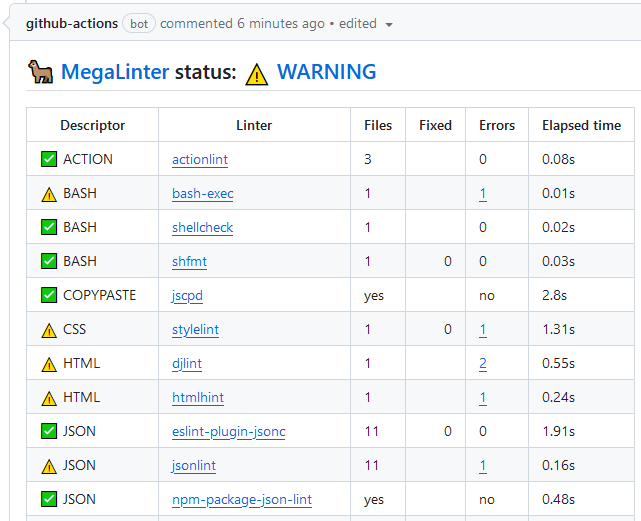
\includegraphics[width=\textwidth]{figures/megalinter_report.png}
\end{figure}

\begin{figure}
  \centering
  \caption{\label{fig:similarity_flamegraph}Flame graph for the similarity endpoint. Most time is spent in matrix maths functions}
  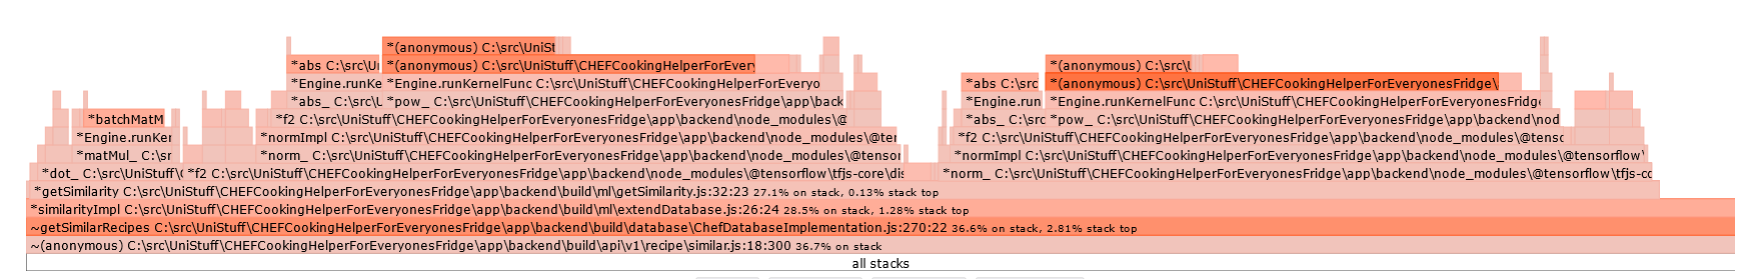
\includegraphics[angle=90,height=0.9\textheight]{figures/similarity_flamegraph.png}
\end{figure}

\begin{figure}
  \centering
  \caption{\label{fig:test_report}A test report showing that some tests have failed.}
  % cSpell: disable
  \begin{verbatim}
mocha --reporter dot --require ts-node/register src/tests/**/*.ts

  ....................!!..................................
  ........................................................
  .........

  119 passing (9s)
  2 failing

  1) /api/v1/signup
        should return a valid token for the new user:

      AssertionError [ERR_ASSERTION]: Expected values to
        be strictly equal:
+ actual - expected

+ 'number'
- 'string'
      + expected - actual

      -number
      +string

      at Context.<anonymous> (src/tests/api/testSignup.ts:50:12)
      at processTicksAndRejections
        (node:internal/process/task_queues:95:5)

  2) /api/v1/signup
        should not allow signing up with an existing username,
        case insensitive:
      Error: expected 400 "Bad Request",
        got 500 "Internal Server Error"
      at Context.<anonymous> (src/tests/api/testSignup.ts:71:8)
      at processTicksAndRejections
        (node:internal/process/task_queues:95:5)
  \end{verbatim}
  % cSpell: enable
\end{figure}

\begin{figure}
  \centering
  \caption{\label{fig:coverage_report}A coverage report showing which lines were and were not executed during test suite.}
  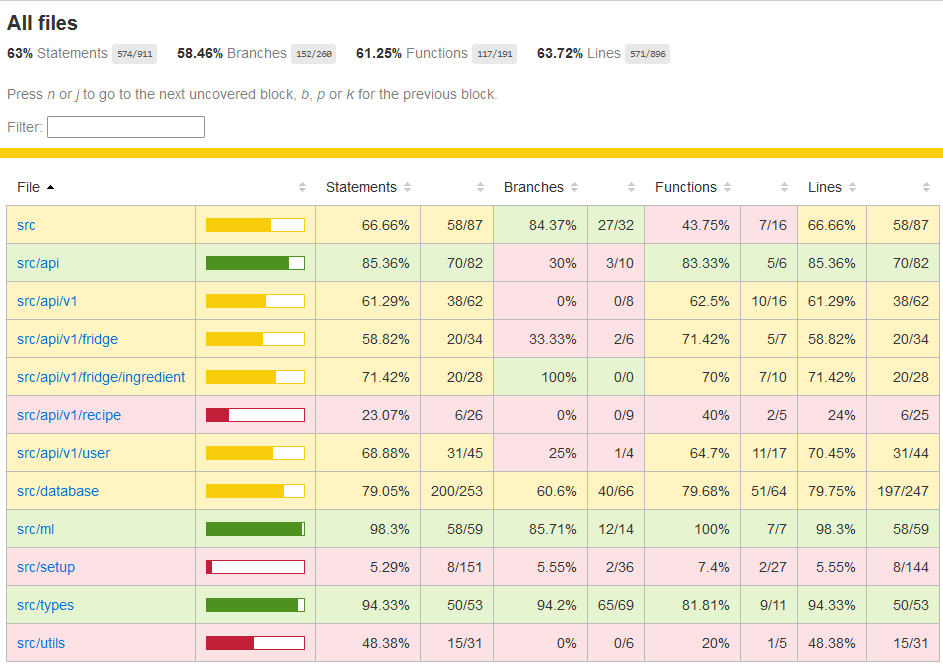
\includegraphics[width=0.9\textwidth]{figures/coverage_report.png}
\end{figure}

\begin{figure}
  \centering
  \caption{\label{fig:test_failure}The email sent if one or more test cases fail.}
  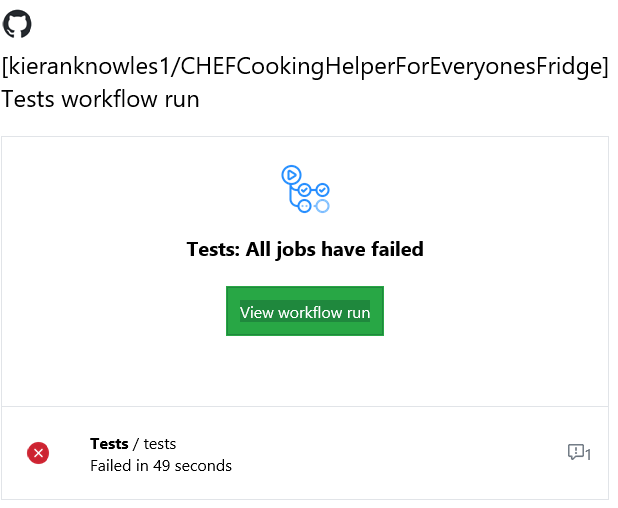
\includegraphics[width=0.9\textwidth]{figures/test_failure.png}
\end{figure}
